\chapter{Study Design and System Implementation}
\label{chapter:studysetting_conduction}
\section{Study Design}
\subsection{Independet Variables: Visual Perspectives}
The last chapter pointed out five possible visual perspecitves in a scenario with one teacher and one student, compare figure~\ref{fig:perspectives}. All visual perspectives are worth an investigation and a comparable study with all five visual perspectives is desirable. Though, to reduce complexity and the number of participants\footnote{Due to COVID-19 pandemic}, this work will focus on three visual perspectives.\\
Figure~\ref{fig:perspectives} shows three main classes of visual perspectives: ego-centric, exo-centric and combinations of them. To answer the research question, it is indispensably to examine at least one of each class. The ego-centric VP is unique and though choosen by default. The exo-centric VP can be realised as purely exo-centric or augmented exo-centric. The combination of ego-centric and exo-centric can be realised as ego \& exo-centric or ego \& augmented exo-centric. But before the exo-centric vp and the combination can be chosen, a closer look on the mechanics that makes Motor Learning in VR possible is necessary.

\subsubsection{Excursion: Mechanics for Motor Learning in Virtual Reality}
For teaching movments in Virtual Reality, in the exo-centric visual perspective the following issue arises. The guidance visualisation can move out of the field of view of the learner by the movement itself. Szenario: the learner and the guidance visualisation stand side-by-side, the learner sees the guidance visualisation on the left of him/her. The guidance visualisation now indicates a movement to turn by 90 degrees to the right. When the learner follow this movement, the guidance visualisation will be located behind the learner after the movement ended. A guidance visualisation standing behind the learner cannot be seen by the learner.\\
This issue is solved in existing work with either the restriction of movements~\cite{freethrowsimulator,elearningma} or multiple representations of the guidance visualisation arround the learner~\cite{thaichichua,mythaichicoaches}. The restriction of movements has an strong influence in the task design and is therefore not desirable for the study proposed in this thesis. Consequentially, for exo-centric visual perspectives multiple representations for the guidance visualisations on strategic positions arround the learner are necessary.\\
In the ego-centric visual perspective, another issue araises during the teaching of locomotion movements. To understand this issue, two aspects have to be clear before. (1) The nature of an ego-centric guidance visualisation is to be located inside the learner at any time. (2) A guidance visualisation indicates movements by moving itself. If the guidance visualisatoin is about to indicate a movement away from the learner, the guidance visualisation is moving out of the students body. But a guidance visualisation that is outside of the learners body is no longer ego-centric.\\
A possible soltuion can give the centricity continuum by Wang and Milgram~\ref{fig:ego-exo-continuum}. Following the nature of the centricity continuum, the tethering distance can be increased by a small ammount and the visual perspective can still be classified as ego-centric. But now araises the question, of how far the tethering distance can be increased, with which the perspective still feels ego-centric, but the indication of the movement is considerable. For simplicity reasons, this distance is further called ego-centric tethering distance (ETD). To determine a reasonable ETD, a small formative study was conducted\footnote{A larger study was not possible because of the COVID-19 pandemic}. During this study, a non biased\footnote{The person had no prior knowledge about the system or motor learning.} person was asked to follow movements in the ego-centric visual perspective. The first movement was conducted with an ETD of 5cm. For the folowing movements the ETD was increased by 5cm each. The subjective assesment of the participant and my observations yielded best for an ETD between 15cm and 30cm. These two values are further called:
\begin{itemize}
	\item[] $ETD_{min}=15cm$
	\item[] $ETD_{max}=30cm$
\end{itemize}
Based on $ETD_{min}$ and  $ETD_{max}$ the speed mechanic is developed. The speed mechanic controls the speed of the playback of the guidance visualisation. At $ETD_{min}$ and below, the animation plays at normal speed. At $ETD_{max}$ the guidance visualisation stops. Between $ETD_{min}$ and $ETD_{max}$ the animation speed of the guidance visualisation is linearly interpolated, compare figure~\ref{fig:speed_mechanic}.
\begin{figure}[htb]
	\centering
	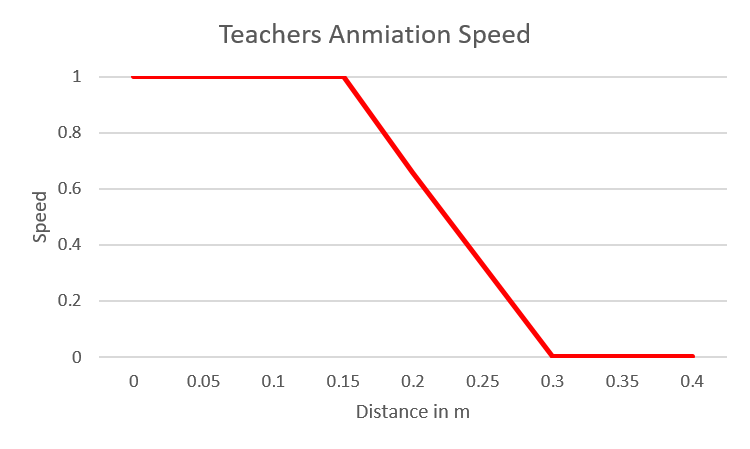
\includegraphics[width=\textwidth]{figures/speed_mechanic_chart.png}
	\caption[speed mechanic chart]{speed mechanic chart}
	\label{fig:speed_mechanic}
\end{figure}
The speed mechanic was evaluated by one person\footnote{Different person than the first one. This person had no prior knowledge about the system nor Motor Learning. A Larger evaluation was not possible because of COVID-19 pandemic.}. The participant followed the guidance visualisation in the ego-centric visual perspective. Observations showed that the participant could follow the movement at ease. The opinion of the participant about the speed mechanic was very positive.\\
With this short excursion, a reasonable decision for the exo-centric VP and the combination can be chosen.\\
\hspace{1cm}

In the ego-centric visual perspective, the learner sees the guidance visualisation inside the own body. Here, the learner can see the relation of the own body to the GV directly. In the pure exo-centric visual perspective this relation cannot be seen. Thereby, the position of the learner in relation to the guidance visualisation must be guessed. That, in turn, makes the application of the speed machanic - which is necessary for ego-centric guidance - not possible. A mechanic that is used in all conditions but one could lead to biased data, compare table~\ref{tab:mechanics}.
\begin{table}[htb]
	\centering
	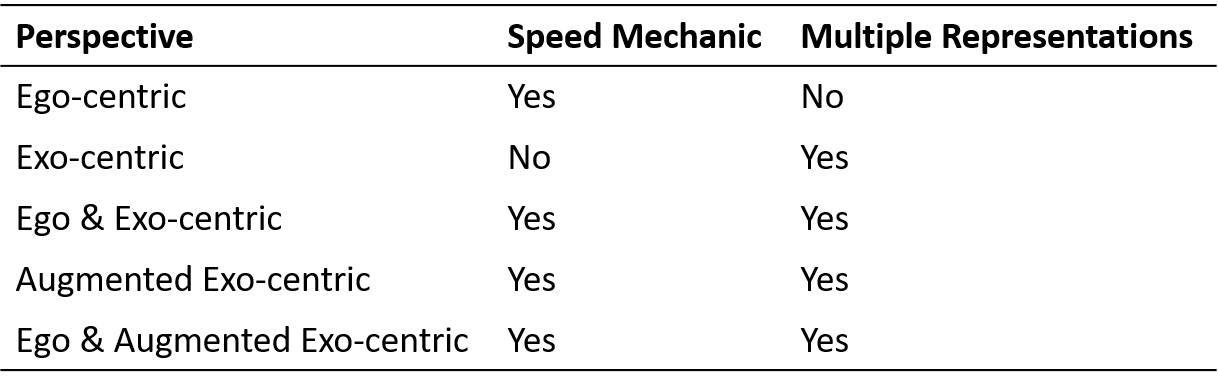
\includegraphics[width=\textwidth]{figures/mechanics_comparison.png}
	\caption[Mechanics for Motor Learing in Virtual Reality]{Mechanics speed and multiple representations and in which VP they are applied.}
	\label{tab:mechanics}
\end{table}
The mechanic of multiple representations does not influence the validity of the study, because the mechanic would solve an issue that does not exist in the ego-centric perspectives.\\
In the augmented exo-centric perspective, a virtual copy of the learner is located inside the exo-centric guidance visualisation. The copy lets the learner see the relation of the own body to the guidance visualisation. Furthermore, augmenting the exo-centric guidance visualisation with the learner is widely used and evaluated in related work~\cite{YouMove,thaichichua}. Consequently, the augmented exo-centric VP will serve as the exo-centric VP.\\
With the ego-centric and exo-centric VP set, the combination can be chosen. In the ego-centric VP the learner has a direct comparison of the own posture to the posture of the GV in the ego-centric VP. In the augmented exo-centric VP the learner has a direct comparison of the own posture and the posture of the GV in the exo-centric VP. To have the direct comparison from the ego-centric VP AND the exo-centric VP, the ego \& augmented exo-centric VP is chosen as the combination. The ego \& augmented exo-centric VP is the true combniation of ego-centric and augmented exo-centric.\\
For simplification, the augmented exo-centric VP will be further called exo-centric VP, and the ego \& augmented exo-centric will be further called ego \& exo-centric VP.\\
The ego-centric VP, exo-centric VP and the ego \& exo-centric VP are the independent variables of the study and form the three study conditions EGO, EXO, EGO \& EXO.

\subsection{Task Design}
Hornb\ae{}k~\cite{hornbaek} identifyed three main typs of tasks in HCI studies: representative tasks, simple tasks and tasks that use task specific hypothesis. RQ1 states the main investigation field is Motor Learning. Motor Learning is strongly related to real-world movements, evidently the study task is a representative task.\\
Real-world tasks that include the handling of physical load, can found in a wide range of activities. For example, a storekeeper job is to clear a palette of cardboard boxes. This task includes to unload the palette, scale the boxes, measure the dimensions of the boxes and finally store them in a rack. Another example is the work at a grinding machine. The worker takes a slug from a shelf and works on it until the sulg becomes a workpiece.  After that the workpiece is carried to a measurement instrument to be varified. There are plenty of other examples, but these two already clarify that a tasks which includes the handling of physical load consitst out of the elemental tasks for manual material handling: lift, lower, push, pull, hold.\\
The idea for the study task is to chain these elemental task together to a Unit-Combined-MMH task, that representatively stand for a wide range of tasks that includes the handling of physcal load. To achieve this, several aspects have to be taken into consideration: (a) the artifacts with which the learner will interact, (b) a reasonable task decomposition that allows the investigation of sub-tasks. Furthermore, the study needs a (c) structure. (c) will reveal the necessity of three tasks. These tasks have to be equally (d) complex. This section will subsequently discuss (a-d) and propose the task for the study.

\subsubsection{(a) Artifacts}
A task that include the handling of physical load obviously need a physical load. In real-world tasks, the physical load can be everything a human can handle. The physical load for this task should fulfil the following criteria: the load should have a significant weight, that it is actually percepted as a load, but at the same time, any healty person with no previous illneses can handle it without getting injured. Secondly, the physical load should give a enough freedom for interactions. A simple box fulfils the criteria and furthermore has a relation to physical loads of real-world tasks like the handling of parcels. With a physical load, the elemental tasks of lift and lower can be realised by lifting and lowering the box from and to the floor.\\
Push and pull can be realised by pushing and pulling the box on the floor, but it can feel cumbersome. Moreover, in real-world task pushing and pulling a box is made possible in a more ergonomic height if possible, not least for security reasons. To support push and pull, a table is introduced. This table stands representatively for example the grinding machine or a parcel sorting table.\\
Finnaly, the transitions between the elemental tasks have to be supported, to increase the real-world reference. This is achieved by providing a waypoint. The waypoint is a plate on the floor and helps to brings sence in movements. This plate representatively stands for example for a scale or second machine. Walking to a scale or lower a box to the scale on the floor increases the real-world reference more than just an empty place in the room.

\subsubsection{(b) Sub-tasks}
The goal is to create a Unit-Combined-MMH task with the elemental tasks push, pull, lift, lower and hold. The process of desining the task is complex and happend iteratively.\\
In the first approach, was a task with four ocuurences of every elemental task. For lifting the box from the scale and carry the box to the table, obviously a new task type had to be introduced: carry. Because carry is not a elemental task and for simplicity, elemental tasks and newly introduces task types are from now on referred as sub-tasks. This first approach of designing a task revealed an issue: chaining a given amout of sub-tasks together so that the task is still conductable is hard to achieve. To overcome the inflexebility, a new sub-tasks is introduced: walk. Walk means locomotion without the box in hand. With walk, the box can be pushed from one side of the table, and then be pushed from the other side of the table, which achieves flexibility in task design, otherwise on push will always follow pull.\\
The next approach was a task that consists out of the sub-tasks push, pull, lift, lower, carry, walk and hold. Each sub-task appeared again four times. The task was evaluated with one person. This person had to follow the instructions in the ego-centric VP and exo-centric VP. During the conduction of the task, the person started to look around and correct the own position during the sub-task hold. An interview afterwards showed, that the person thought the GV stopped because his position was too far away from the GV. It became clear, that the speed-mechanic and the sub-task are not compatible. For the participant of the study it is indistinguishable if he/she is to far away from the GV of if it is the sub-task hold. Because of this indistinguishableness, the sub-task hold is excluded from the task as sub-task. However, hold is still part part of the whole tasks: between the transitions of the tasks (for example between lift ends and lower starts) is a small pause which is equivalent to hold, but this sequence is to short to log. Furthermore, hold is part of the sub-task carry, where the box is holded in front of the body. But hold is not a stand alone sub-task and connot be evaluated isolated.\\
A new task was desinged with the sub-tasks push, pull, lift, lower, carry and walk. During the design special attention was payed to the magnitide of the movements. For example, every push should be equally far. Lift and lower from and to the scale and lift and lower from and to the table are very diffrent in the magnitude. This resulted in two new sub-tasks: pick and place. Pick means to pick up the box from the table, place means to place the box on the talble, while lift and lower the targed remained the scale on the floor.\\
The next stage of the task consits out of the sub-tasks push, pull, lift, lower, carry, walk, pick and place. The task was inspected by an professional physiologist. The physiologist was asked to describe the sub-tasks in detail and perform every sub-task ergonomically. The professionals description of the sub-tasks are listed in table~\ref{tab:sub-tasks}. From the performance of the professional physiologist and the description of the sub-tasks could be derived several insights. The sub-tasks push and pull are very similar in their conduction. The same applies for the pairs lift and lower as well as pick and place. This meant for the evaluation, that the variations of movements is nearly halfed, and the possibility of making mistakes is reduced. Example: for push and pull, one foot has to be placed to the back while the other foot remains under the hip, the hands do the same for every push and pull. If in the participant does perform the sub-task intrinscally correct without the perception of the GVs, the study wil not meassure the influence of the perspective. To increase the number of sources of error, two new sub-tasks are introduced: turn and fold. Turn means to turn the box by 90 degrees on the table, fold means to tilt the box from one side to another. The difference of the hand movement to push and pull is obvious. The difference for the feet results from the fact, that during turn and fold, the weight of the box remains on the table and the force to apply on the box is significantly lower than during push and pull. This results in a different feet placement, which are hip wide under the hip.\\
The introduction of turn and fold all sub-tasks are introduced. A new task was created with all 10 sub-tasks. To assess all sub-tasks multiple times, they appear four times per task. The pair lift and lower and the only in magnituded diffrent pair place and pick realate to each other. To be presented equally in the task among the other sub-tasks should also only be present four times. Because, lift and lower are measured with the RM (6.2) (see next section) lift and lower was decided to appear three times each, and pick and place one time each. Unfortunately, only one time each pick and place meants that all sub-tasks that do not happen at the table had to be conducted in seuquence. To regain flexibility in the task, it was decided that pick and place will occur 2 times each. This results in 34 sub-tasks per task. Table~\ref{tab:sub-tasks} provides an overview over the sub-tasks and their corresponding description, as well as the occurences per task.

\begin{table}[H]
	\centering
	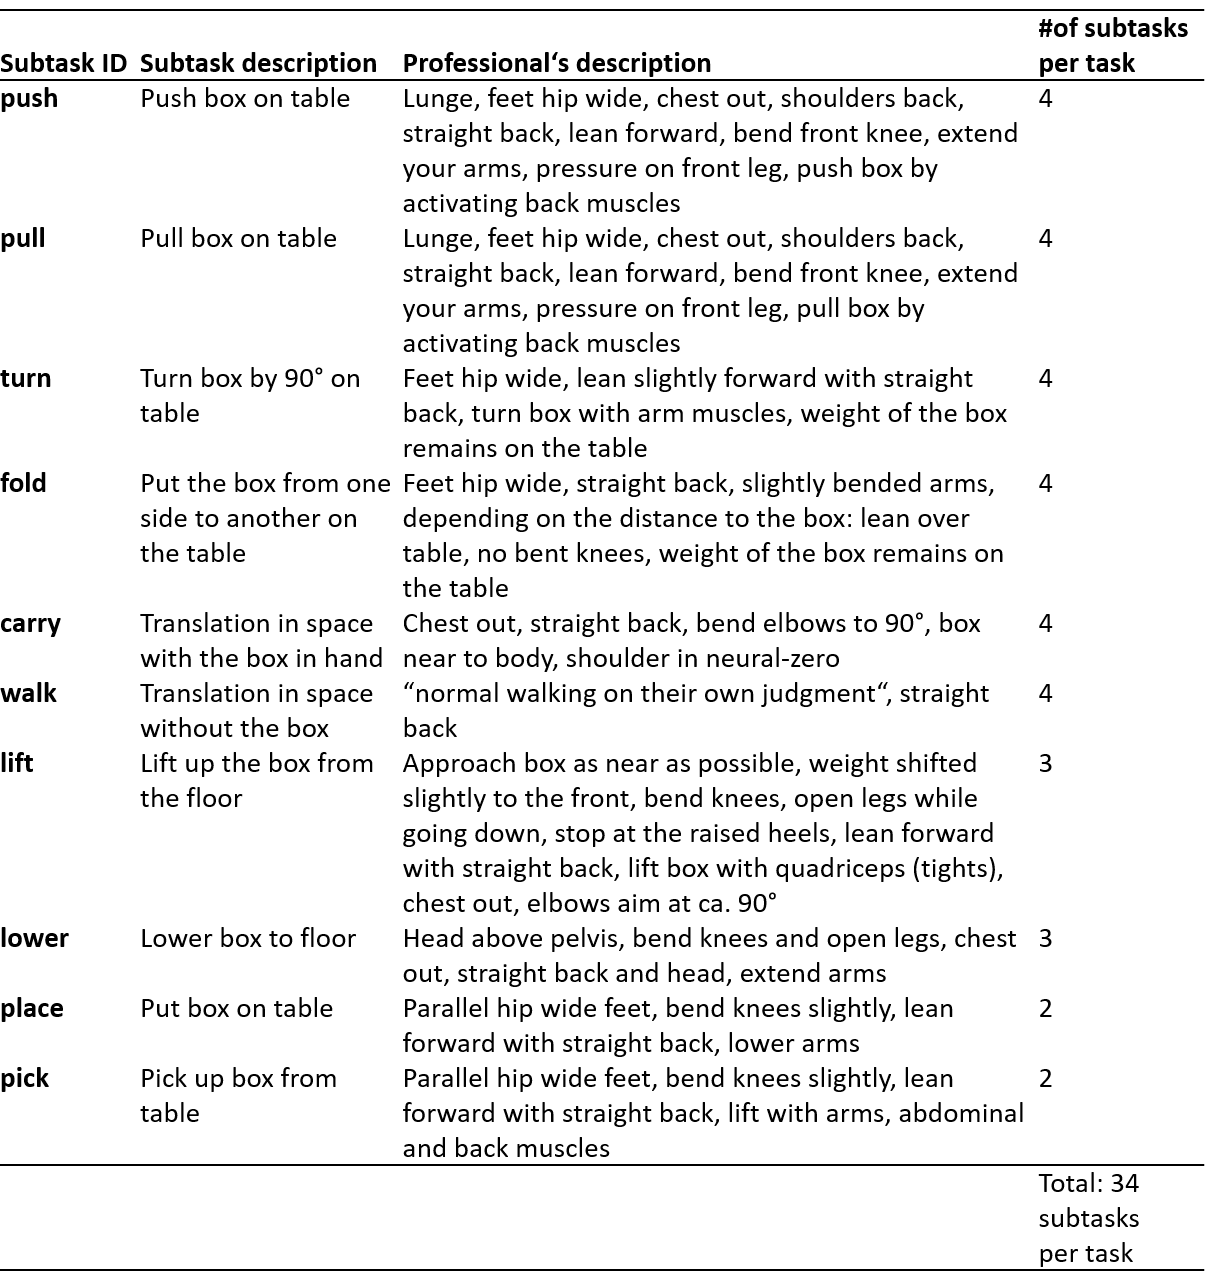
\includegraphics[width=\textwidth]{figures/sub_tasks_definition.png}
	\caption[Description of sub-tasks]{Sub-tasks that appear in every task.}
	\label{tab:sub-tasks}
\end{table}

\subsubsection{(c) Study Structure}
In the study three conditions are compared: EGO, EXO and EGO \& EXO. The main question in this section is how to assign the participant to the independent variables. The key destincting is between within-subject design and bewteen-subject design~\cite{hornbaek}. In the within-subject design the participant would experience all VPs. In the between-subject design, the participants would experience only one VP. Within-subject desings typically can detect the differences of between the conditions more precisely, ibid.. Furthermore, within-subject designs need less participants~\footnote{The COVID-19 pandemic makes it hard to find enough participants.} than between subject designs, ibid.. For these reasons, is conducted in a within-suubject design. The within-subject design does also have a drawback: the participants gain experience about the task and the conditions during the study. This means that one condition is influence by another condition, which the participant already experienced. Furthermore, there is a asymetrical carry-over effect between the conditions: EGO \& EXO contains condition EGO and EXO and thereby influences EGO and EXO more than EGO influences EGO \& EXO. To reduce the task related learning effect, three tasks with an nearly equal complexity is created. With this, a participant will face for every condition a different task. The tasks are still similar and the learning effect persits. A reduction of the influence of the learning effect on the outcome can be countered out by counterbalancing the task. Similar to the task, the carry-over effect between the conditions can be also countered by counterbalancing the conditions. Hornb\ae{}k proposes in this case to cross the conditions with the task and use a Greco-Latin square. Three conditions and three tasks in a Greco-Latin square results in blocks of nine participants. This block is depicted in figure~\ref{fig:study_session_plan}. The study should be conducted with at least 4 blocks (4x9=36 participants) \todo{warum?????}.

\begin{figure}[htb]
	\centering
	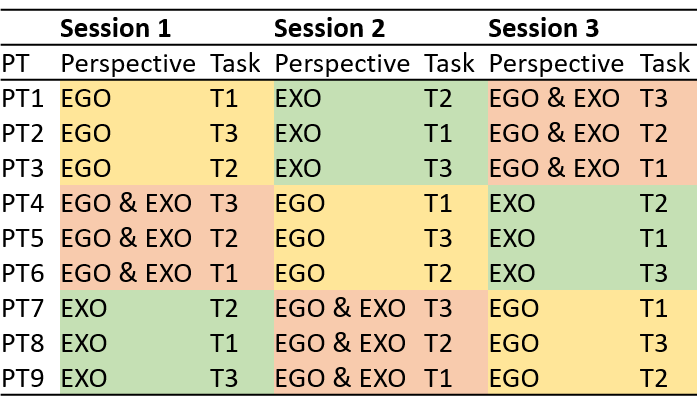
\includegraphics[width=0.5\textwidth]{figures/study_session_plan.png}
	\caption[Study structure]{Experiment structure: within-subject desing in a Greco-Latin square.}
	\label{fig:study_session_plan}
\end{figure}

\subsubsection{(d) Equal Task Complexity}
A study participant will face in every condition another task. For the validity of the study it is indispensable that these three tasks have a nearly equal complexity. As described in (b) a task consits of 10 subtasks that occur a specific amount. The main idea to ensure a comparable complexity is to to use the for all three tasks the same sub-tasks in an equal amount. This means, the 34 sub-tasks of task one occure in task two and three, but in a different order. Table~\ref{tab:tasks} lists all three tasks. For every task, the a sub-task number ST1-ST34 is provided. Every number stands for a sub-tasks, which comes with a description and the sub-task ID. Reading the description from top to bottom are the instructions the learner recieves from the GV during one condition. The mirror mention in the first line is another waypoint which. The mirror is necessary for technical reasons and is described in section \todo{4}.

\begin{table}[H]
	\centering
	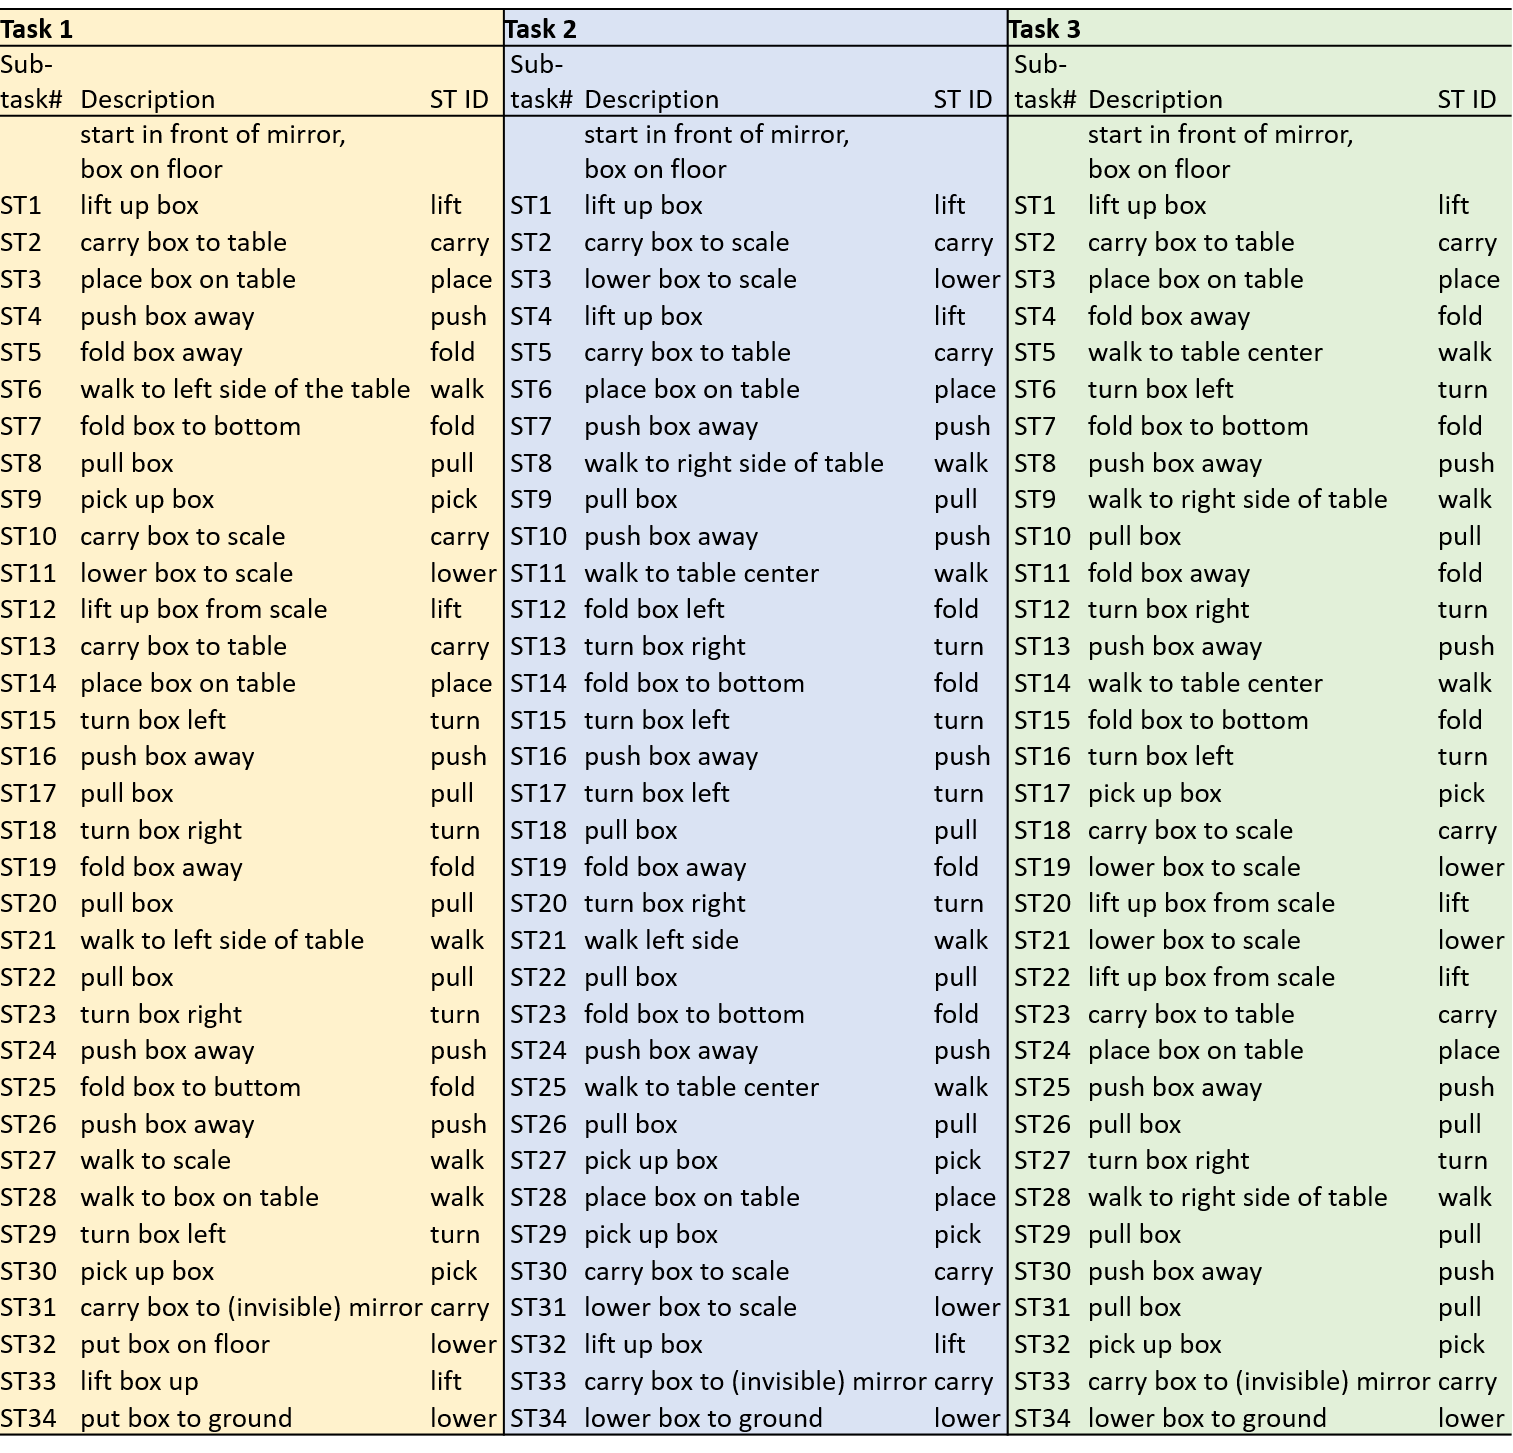
\includegraphics[width=\textwidth]{figures/tasks.png}
	\caption[Description of tasks]{tasks}
	\label{tab:tasks}
\end{table}

\subsection{Measures: dependent variables}
This works aim is to answer the main researchquestion RQ1: How does the visual perspective on a virtual guidance visualisation influence Motor Learning in Virtual Reality. To answer this research question, the proposed study has to generate data that answers the sub-research questions RQ1.1-4. This section will provide the underlying paradigma to every sub-research question and explain which measures are necessary.\\

\textbf{RQ1.1} How does the visual perspective on a virtual guidance visualisation influence movements' accuracy?\\
\textbf{Paradigma:} the more exact the learners movements maches the GV movements, the better the learner could follow the instruction of the GV. For RQ1.1.1 the limbs of the learner and the limbs of the GV are compared. For RQ1.1.2 the box' accuracy is compared. For RQ1.1.3, both are compared and addiionally, the current sub-task is taken into consideration. The accuracy can indicate, how the particular movement is suited for the VP.
\begin{itemize}
	\item[] \textbf{RQ1.1.1} How does the visual perspective on a virtual guidance visualisation influence movements' accuracy of the own body?\\
	\textbf{Measures}: (1) Euclidean distance between the learners and GVs hands, feet, head and hip in meters. (2) Angle between learners and GVs the hands, feet, head and hip in degrees.

	\item[] \textbf{RQ1.1.2} How does the visual perspective on a virtual guidance visualisation influence the accuracy of handling physical load?\\
	\textbf{Measures}: (3) Euclidean distance between the learners and GVs phsical load. (4) Angle between the learners and GVs physical load in degrees.

	\item[] \textbf{RQ1.1.3}How does the visual perspective on a virtual guidance visualisation influence sub-tasks' accuracy?\\
	\textbf{Measures}: (1-4), additionally matched to the sub-tasks that is currently performed (5).
\end{itemize}	
(1-4) gives insights to what extend the learner could follow the GV for the whole task. (5) can extract specific sub-tasks for which the learner could follow the GV to a certain extend. For example, in the ego-centric VP the overall accuracy for a task is lower than in the other VPs, but the accuracy for the sub-tasks lift and lower is higher than in other VP. For this example, measure (5) can extract specific sub-tasks that are performed better or worse than in other VPs.\\

\textbf{RQ1.2} Does the visual perspective on a virtual guidance visualisation influence the transfer of ergonomic principles?\\
\textbf{Paradigma:} the more exact the learners RM matches the GVs RM, the better the ergonomic principles could be transfered.\\
\textbf{Measures:} (6) Risk Measurements: (6.1) spine bend in degrees, (6.2) squat distance in meters, (6.3) good base in meters \todo{check names}, (6.4) box near body.\\
Muckell et al.~\cite{muckell} used four RM in their work to assess the perofrmance of the conducted movements. Three of them are assessed in the proposed study, too.
\begin{itemize}
\item[] (6.1) spine bend is defined by the difference in degrees between the straight upward vector and the back of the learner. For all sub-task, spine bend schould be in a certain window. This window is calculated form the teacher, who recorded the movement. Spine bend indicates, if the learner could percept the correct posture of his back.

\item[] (6.2) squat distance is defined by the distance in meters between the feet. For the sub-tasks lift and lower, the squat distance schould be in a certain window. This window is calculated form the teacher, who recorded the movement. For the other sub-tasks, squat distance is not applied. Squat distance indicates, if the learner could percept that he should bend his knees during lift and lower.

\item[] (6.3) good base is defined by the distance in meters between the feet. For the sub-tasks push, pull, turn, fold, lift, lower, pick and place, the squat distance schould be in a certain window. This window is calculated form the teacher, who recorded the movement. Good base indicates, if the learner could percept the correct posture of the feet.
Muckell et al.\cite{muckell} use the RM spine bend in their work. This RM cannot be applied for this study because of the multiple perspective mechanic. The learner has mulitiple GV around him/her and is free of choice which one to look at. The turn of the head implies spine twist. Though, spine twist has a low validity and reliability.

\item[] (6.4) box near body. For the study task design, a profesional physiologist was consulted (compare \todo{section}). During the interview, all movements were described in detail, compare \todo{figure}. During the sub-task carry the box should be as near as possible to the body while the elbows should have bend angle of 90 degrees. Unfortunately, the bend angle could not be determined during a study for technical reasons, see chapter \todo{implementation}. Fortunately, the distance from between the box and the body can be determined. Box near body, is defined as the distance in meters between the box and the body of the learner. For the sub-task carry, box near body should be in a certain window. The window is calculated by from the teacher who recorded the movement.
\end{itemize}

RM (6.1-4) are different from accuracy measurements (1-5), because they are independent from the position of the learner and the GV. For example, in the exo-centric VP, a learner cannot percept the correct position where he/she should stand. The learner thereby stands 15cm away from the position he/she should stand. The overall accuracy is thereby lower. But the learner could percept the positioning of his/her feet correctly. In this case the RM (6.3) are fulfiled while the accuracy is biased.\\

\textbf{RQ1.3} How does the visual perspective on a virtual guidance visualisation influence the learner's visual focus?\\
Measures: (7) looking at\\
Paradigma: the learners visual focus is on the object the learner is looking at.\\
The learner interacts with a box and has multiple GVs around and inside the learner. Looking at can give insights on which GV the learner is focusing, the frequency of focus changes and the role of the physical load.

\textbf{RQ1.4} What is the subjective personal preference of the learner for the visual perspectives?\\
Measures: (8) qualitativ data; likert scales, semi-structured interview, digging into occurences.\\
The qualitative data serves not only to investigate the learners personal preference, but can be also serves as triangulation method for measures (1-7).\\

The last measure is the (9) task completion time measured in seconds. The speed-mechanic regulates the speed of the animation of the GV. The further the learner is located to the GV, the slower the animation speed of the GV until it stops completely. The task completion time gives insights about the learning effect \todo{schreib das morgen nochaml}


\subsection{Procedure}



\subsection{How to Evaluate}

\subsection{Research Contribution Statement}
\label{delimination_contribution}
The conduction of the proposed study will produce data that serves as a reasonable basis for designers of VR Motor Learning systems choosing a suitable perspectives. This is achieved by an Empirical Research Contribution. The empirical data is gathered by a comparative study between the ego-centric visual perspective, the exo-centric visual perspective and the combination. As novelty, the task includes handling of physical load which consists of the elemental tasks of manual material handling. This allows an evaluation of the elemental tasks per visual perspective and can give insights which perspective is suited for specific tasks.\\
Additionaly, an artifact contribution is provided by the ego-centric guidance of locomotion movements.
\section{\exgo - Design and Implementation}
(15 pages)
\section{\exgo}
\label{section:system}
\subsection{Study Setting}
Studysetup\\
frameworks\\
implementation\\
perspectives\\
mechanics\\
logging\\
limitations\\
iterative implementation\\
formative tests\\
\section{Study}
\label{section:study}

\begin{figure}[htb]
	\centering
	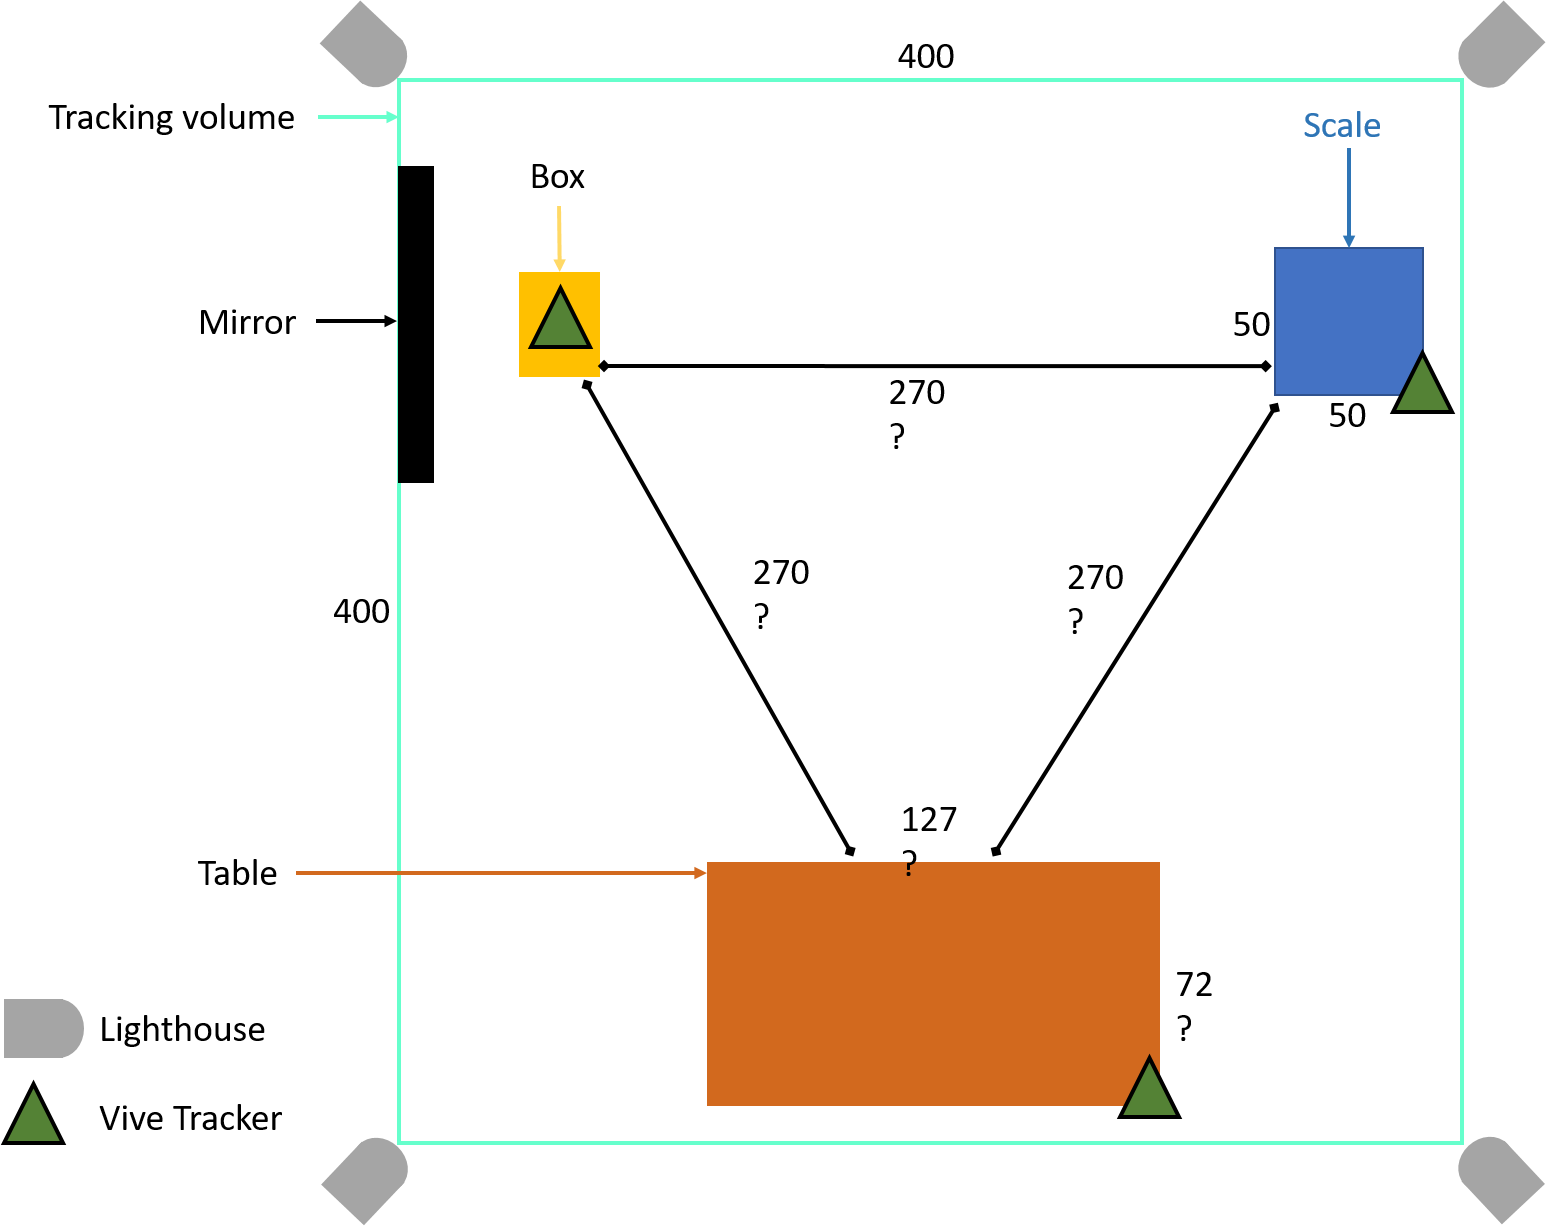
\includegraphics[width=\textwidth]{figures/study_setting.png}
	\caption[study setting]{study setting}
	\label{fig:study_setting}
\end{figure}

\begin{figure}[htb]
	\centering
	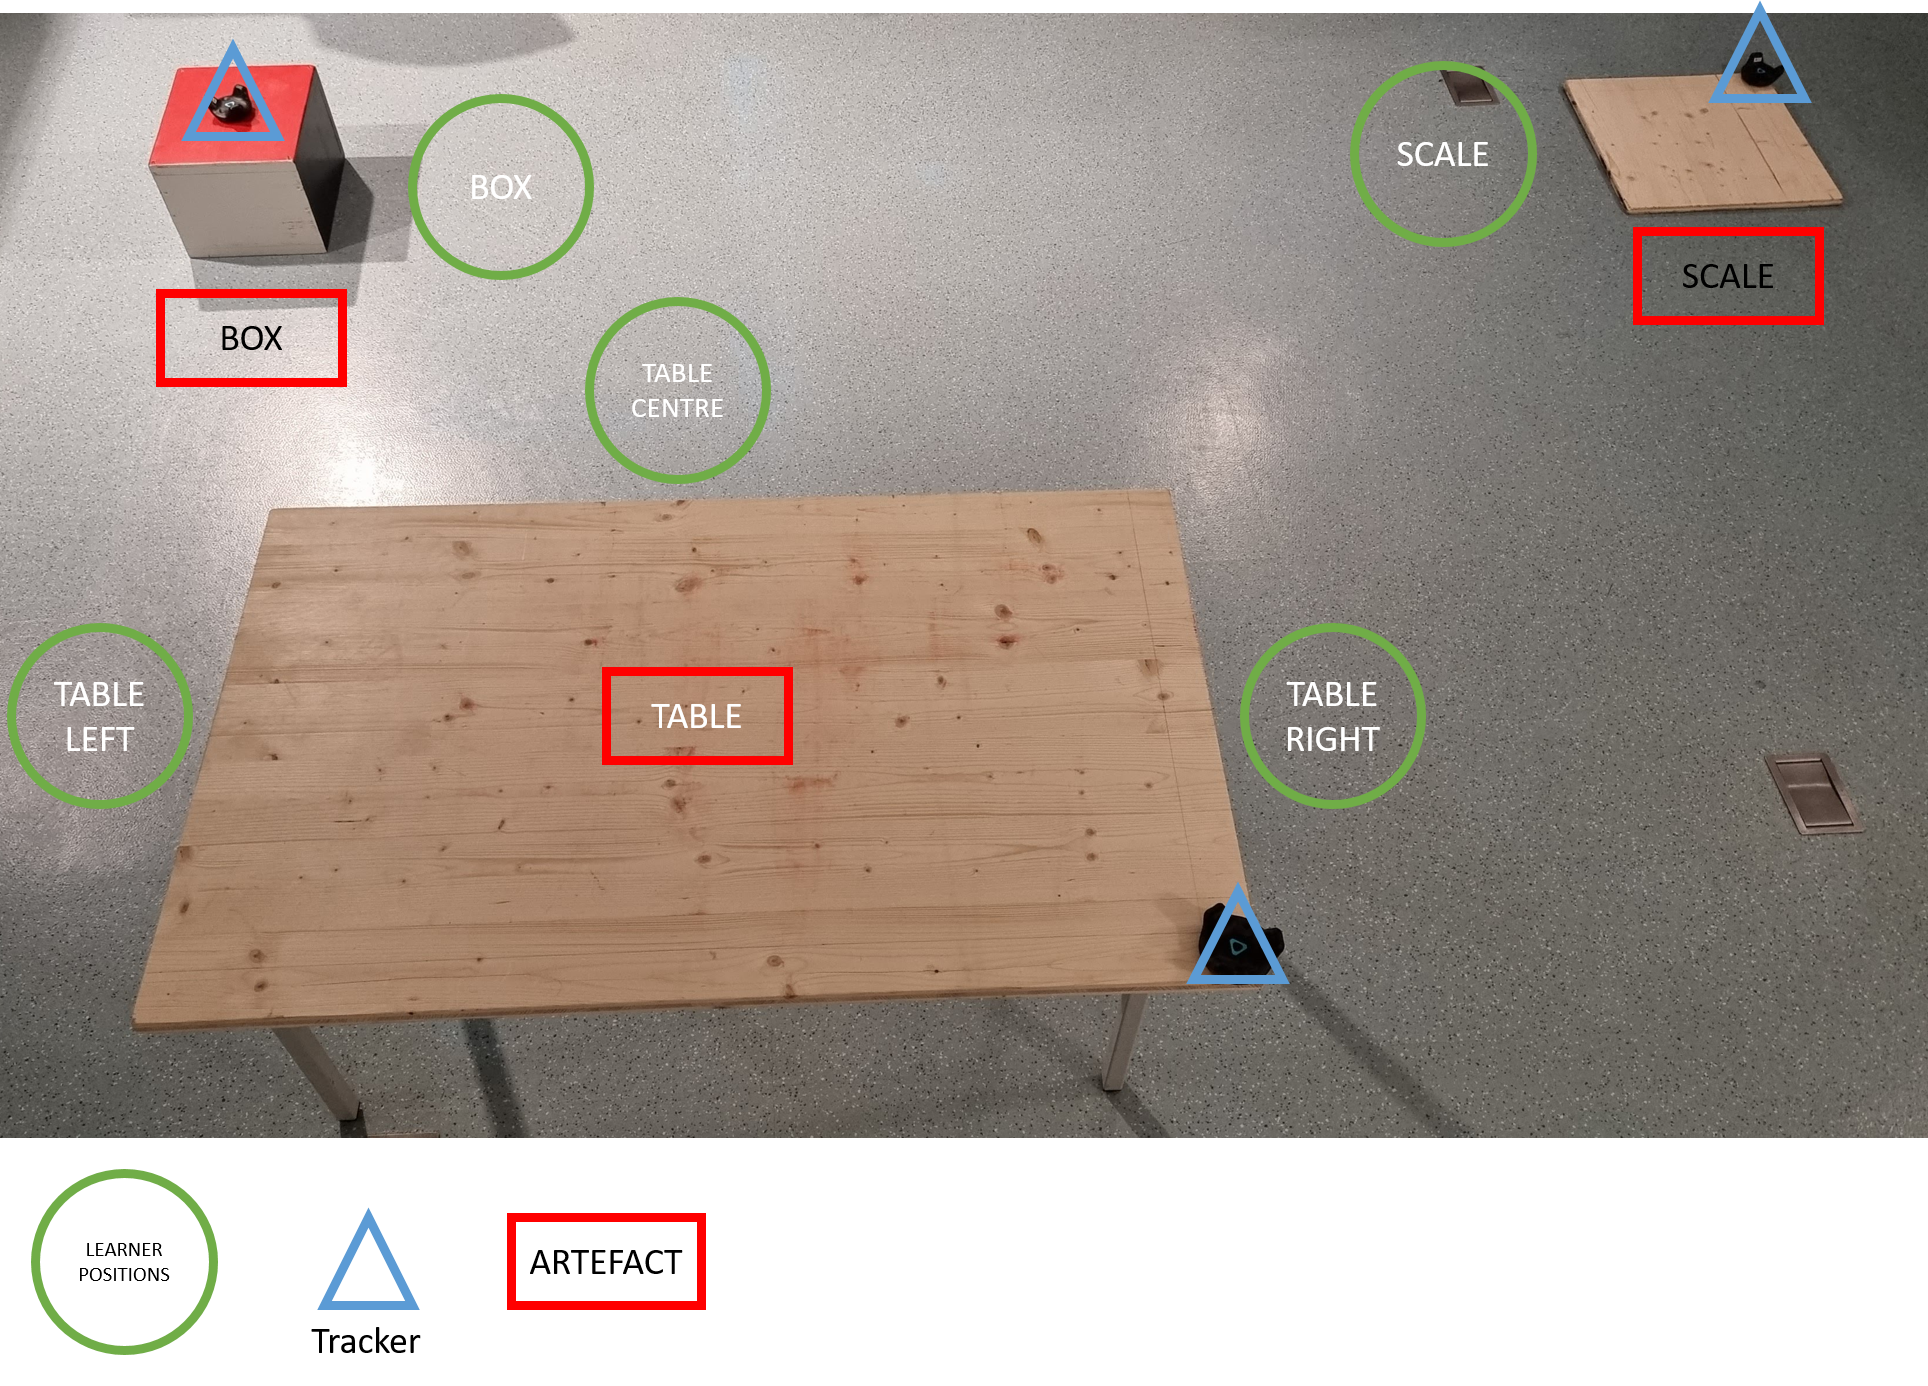
\includegraphics[width=\textwidth]{figures/learner_positions.png}
	\caption[learner positions]{learner positions}
	\label{fig:learner_positions}
\end{figure}

\begin{figure}[htb]
	\centering
	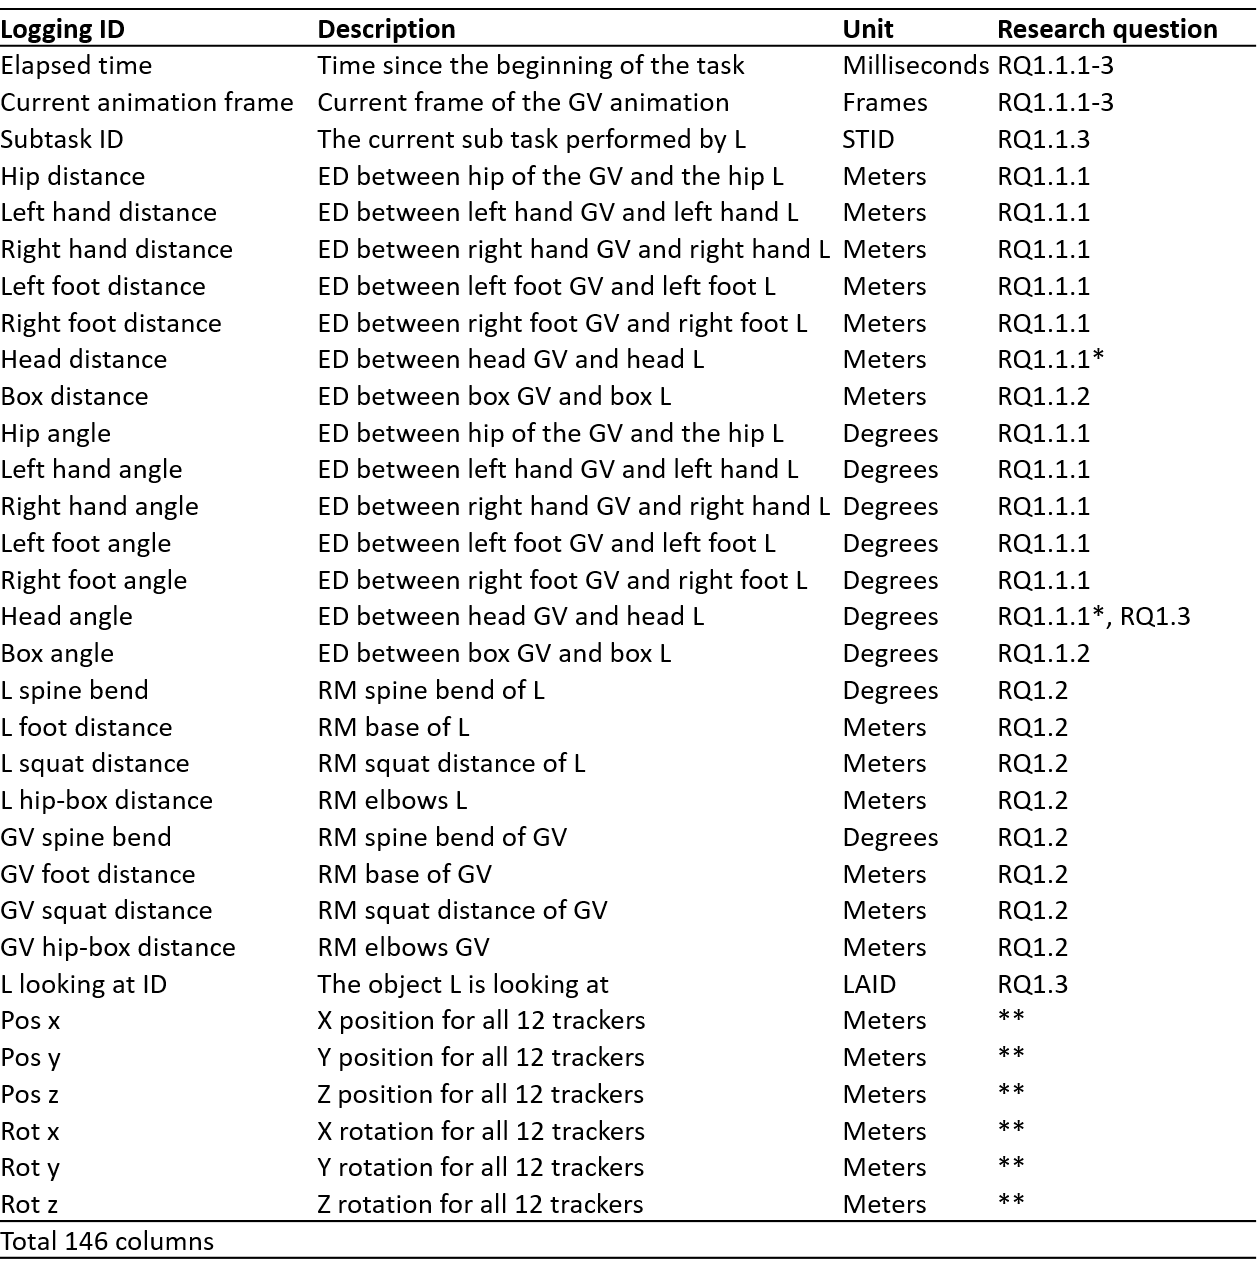
\includegraphics[width=\textwidth]{figures/logging_detail.png}
	\caption[logging detail]{Detailed overview of logs produced by \exgo\ per frame. L: learner, GV guidance visualistion, ED: euclidean distance. *head position and rotation is biased in exo-centric conditions because of multiple GV the L can focus on. **All trackers are logged for backup reasons: after the study is conducted a measurement can become interesting that was not of imporance before. With these values any measurement can be calculated post-study.}
	\label{fig:logging_detail}
\end{figure}





\begin{figure}[htb]
	\centering
	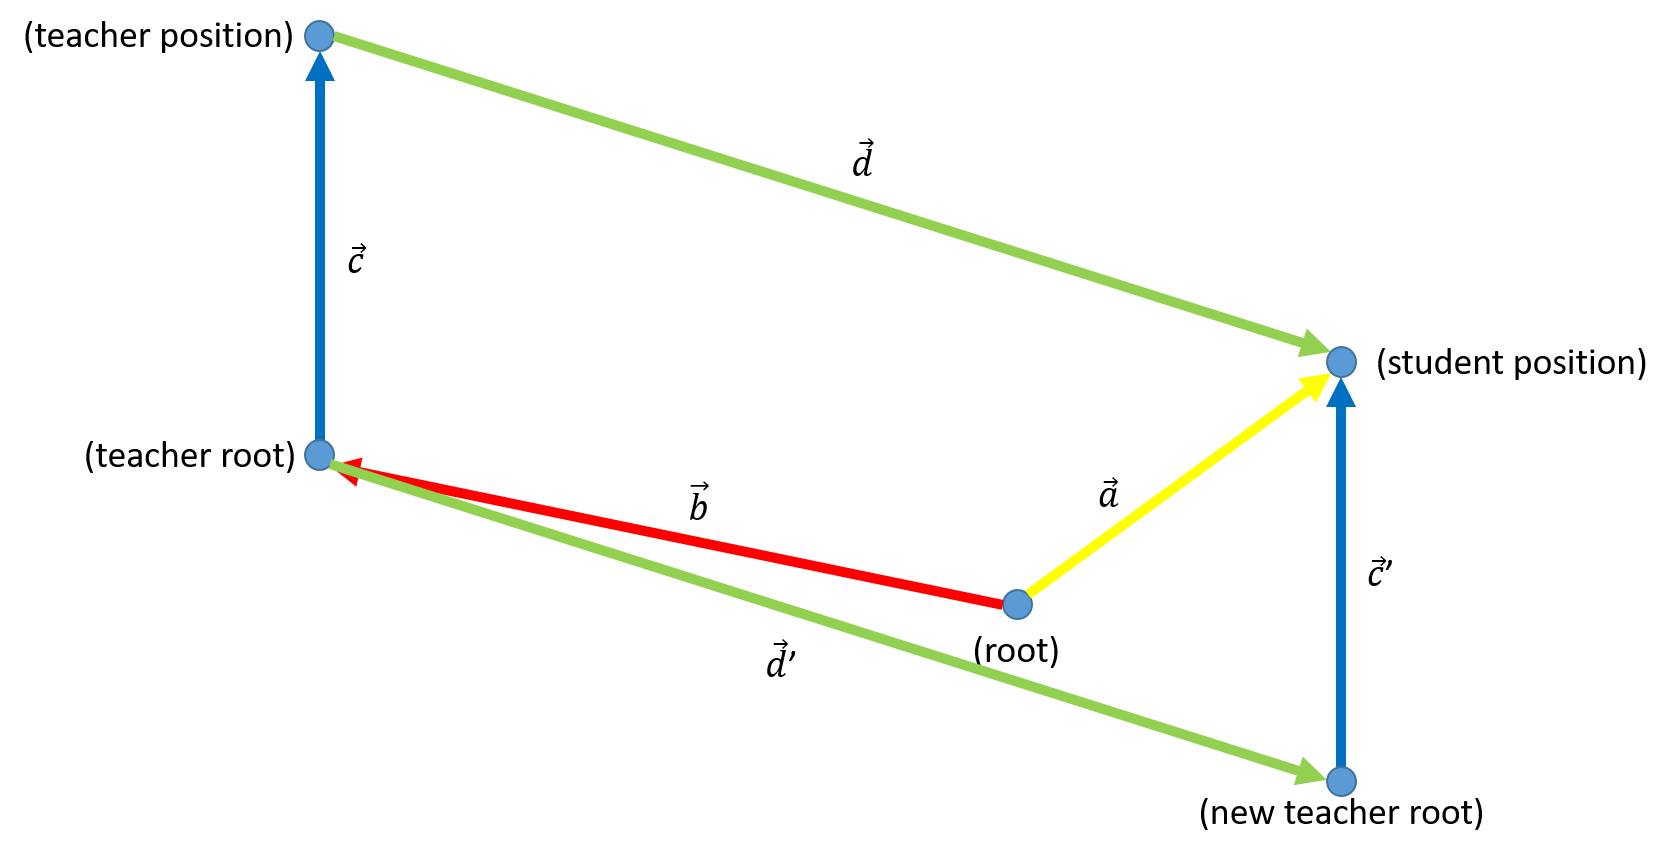
\includegraphics[width=\textwidth]{figures/shift_calc.png}
	\caption[shift calc]{shift calc}
	\label{fig:shift_calc}
\end{figure}





tasks\\
procedure\\
geplante evaluierung\\
limitations\\
bezug zwischen messungen und forschungsfragen\\
triangulation nutzen wo sinnvoll\\
